\documentclass{article}
\usepackage{tikz}
\usetikzlibrary{arrows.meta,positioning,calc,shapes.geometric}
\pagestyle{empty}
\begin{document}
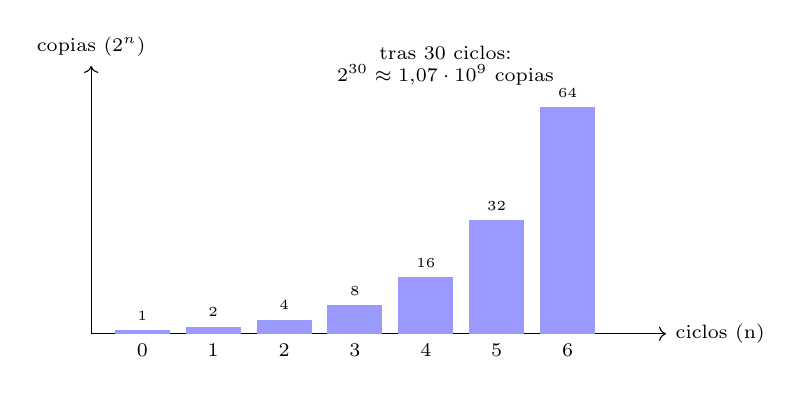
\begin{tikzpicture}
\tikzset{every node/.append style={align=center}}
\draw[->] (0,0) -- (0,3.4) node[above, font=\scriptsize] {copias (2$^n$)}; \draw[->] (0,0) -- (7.3,0) node[right, font=\scriptsize] {ciclos (n)};\fill[blue!40] (0.30,0) rectangle (1.00,0.045); \node[font=\tiny, above] at (0.65,0.045) {1};\fill[blue!40] (1.20,0) rectangle (1.90,0.090); \node[font=\tiny, above] at (1.55,0.090) {2};\fill[blue!40] (2.10,0) rectangle (2.80,0.180); \node[font=\tiny, above] at (2.45,0.180) {4};\fill[blue!40] (3.00,0) rectangle (3.70,0.360); \node[font=\tiny, above] at (3.35,0.360) {8};\fill[blue!40] (3.90,0) rectangle (4.60,0.720); \node[font=\tiny, above] at (4.25,0.720) {16};\fill[blue!40] (4.80,0) rectangle (5.50,1.440); \node[font=\tiny, above] at (5.15,1.440) {32};\fill[blue!40] (5.70,0) rectangle (6.40,2.880); \node[font=\tiny, above] at (6.05,2.880) {64};\node[font=\scriptsize, below] at (0.65,0) {0};\node[font=\scriptsize, below] at (1.55,0) {1};\node[font=\scriptsize, below] at (2.45,0) {2};\node[font=\scriptsize, below] at (3.35,0) {3};\node[font=\scriptsize, below] at (4.25,0) {4};\node[font=\scriptsize, below] at (5.15,0) {5};\node[font=\scriptsize, below] at (6.05,0) {6};\node[font=\scriptsize, align=center] at (4.5,3.4) {tras 30 ciclos:\\ $2^{30} \approx 1{,}07\cdot 10^{9}$ copias};
\end{tikzpicture}
\end{document}
